\subsection{Insertion sort}

\begin{table}[h]
	\begin{center}
		\begin{tabular} { >{\centering\arraybackslash}m{3cm} | >{\centering\arraybackslash}m{2cm} | >{\centering\arraybackslash}m{2cm} }
			\hline
			\textbf{Language}	& \textbf{Time} & \textbf{Ratio} \\ \hline
			C\#					& 0.078s 		& 1:1 \\ \hline
			Java				& 0.131s 		& 1:1.7 \\ \hline
			Python				& 12.525s 		& 1:160 \\  \hline		
		\end{tabular}
	\end{center}
	\caption{Results of the insertion sort test.}
	\label{table:insertion_sort}
\end{table}

Table \ref{table:insertion_sort} illustrates the time it takes for each language to sort 10'000 positive integers in random order. Notice the time differences between Python and the other two languages.

\begin{figure}[h]
	\centering
	\mbox{
		\subfigure[Test results for Insertion Sort in Java and C\#.]{
			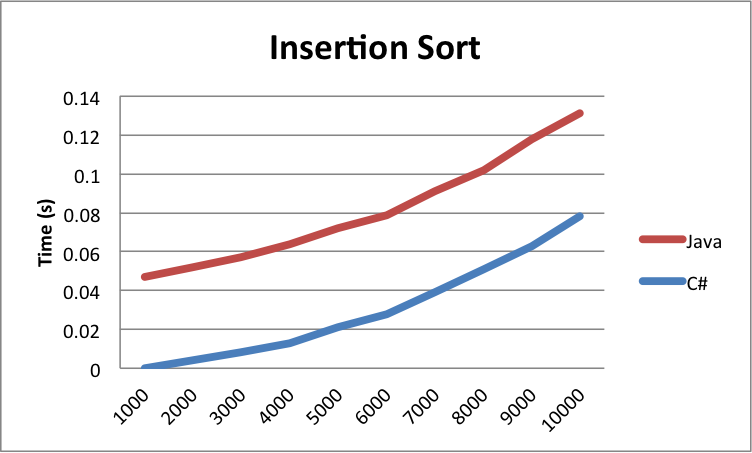
\includegraphics[width=0.48\textwidth]{chapters/media/insertion_sort_csharp_java.png}
			\label{fig:insertion_sort_csharp_java}
		}
		\subfigure[Test results from Insertion Sort in Python.]{
			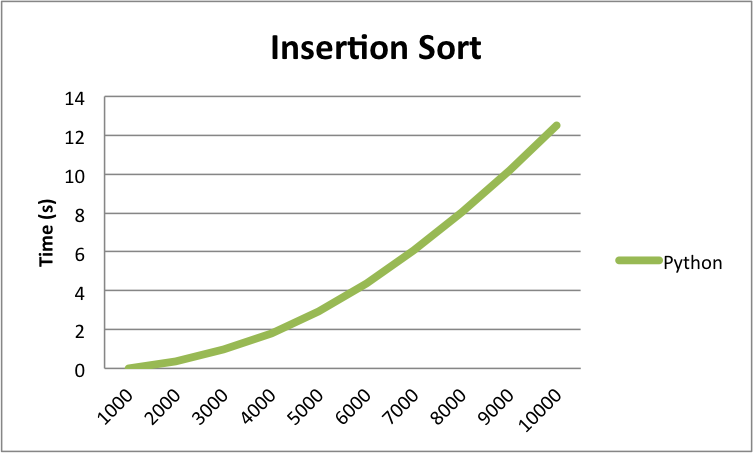
\includegraphics[width=0.48\textwidth]{chapters/media/insertion_sort_python.png}
			\label{fig:insertion_sort_python}
		}
	}
	\caption{Test results for Insertion Sort in C\# and Java to the left and Python to the right.}
	\label{fig:insertion_sort_results}
\end{figure}

Figure \ref{fig:insertion_sort_results} illustrates the relation between the number of positive integers in random order (horizontal-axis) and the time (vertical-axis), it appears to run in $O(n^2)$ under every language. It would appear that Python demonstrates a curve more similar to a quadratic curve. This is because the Stopwatch has better precision the longer it takes to sort the numbers.